\documentclass[10pt]{article}

\usepackage[accepted,preprint]{tmlr}

% ---- 收紧标题与浮动体的垂直间距(必须在 tmlr 之后加载,否则被覆盖) ----
\usepackage{titlesec}
\titlespacing*{\section}{0pt}{1.2ex plus .2ex minus .2ex}{0.7ex plus .1ex}
\titlespacing*{\subsection}{0pt}{0.9ex plus .2ex minus .2ex}{0.4ex plus .1ex}
\titlespacing*{\paragraph}{0pt}{0.6ex plus .1ex}{1em}

\usepackage{caption}
\captionsetup{skip=4pt, font=small}

\setlength{\textfloatsep}{8pt plus 2pt minus 2pt}
\setlength{\intextsep}{8pt plus 2pt minus 2pt}
\setlength{\floatsep}{8pt plus 2pt minus 2pt}
\setlength{\abovecaptionskip}{4pt}
\setlength{\belowcaptionskip}{2pt}

\usepackage{tikz}
\usetikzlibrary{shapes, arrows, positioning, fit, calc}
\usepackage{float}
\usepackage{hyperref}
\hypersetup{colorlinks=true, linkcolor=black, citecolor=black, urlcolor=black}
\usepackage{url}
\usepackage{graphicx}
\usepackage{booktabs}
\usepackage{amsmath}
\usepackage{amsthm}
\usepackage{algorithm}
\usepackage{algpseudocode}
\usepackage{xcolor}

\newtheorem{lemma}{Lemma}
\newtheorem{corollary}{Corollary}

\title{\large DNS++: A Privacy-First, Dynamic, Location-Aware Name Resolution System\\
\large --- A Real-System Implementation and Empirical Evaluation}

\author{\name Shangqing Xu \\
      \addr UCL Department of Electronic and Electrical Engineering}

\def\month{09}
\def\year{2026}
\def\openreview{\url{https://openreview.net/forum?id=XXXX}}
\raggedbottom
\begin{document}
\maketitle

\begin{abstract}
The Domain Name System exposes query intent to intermediaries, cannot keep pace with dynamic service changes, and lacks location-aware replica selection. The DNS++ proposal addresses all three through a hierarchical publish/subscribe overlay with homomorphic encryption, but has only been evaluated in simulation. We present the first real-system implementation of the DNS++ broker in C++17 --- a TLV binary protocol, an epoll event loop, Algorithm~1 (Proximity Routing) with a quadrant-based propagation brake, a multi-broker overlay with dynamic Minimum Bounding Hyperrectangle aggregation, and the modified Paillier privacy layer --- and evaluate it over 30 independent trials per configuration with bootstrap confidence intervals. Three findings follow. The propagation brake is far blunter than simulation suggests: in a three-broker tree it buys a 6.9\% reduction in forwarding events while destroying 77\% of correct nearest-replica resolutions, whereas the quadrant cache alone attains a traffic ratio of 1.168 at 0.981 recall. The privacy layer's broker-side cost is bounded and negligible: a homomorphic Match costs 0.0127\,ms against 23.5--59\,ms for endpoint blinding, bounding broker overhead at $S \times 0.0127$\,ms in the number of subscription groups $S$; a paired comparison over 30 trials finds no detectable latency difference ($p = 0.299$). Convergence after replica migration is directional: when a replica moves closer, subscribers converge in a median of 0.42\,ms, five orders of magnitude faster than a DNS TTL; when a replica moves away, the push-only monotone filter provides no convergence at all (0 of 1391 cases). We report this asymmetry, and the plaintext exposure introduced by hash-based subscription grouping, as the principal limitations of the design as implemented.
\end{abstract}

\section{Introduction}
\label{sec:intro}

Every Internet interaction begins with a name resolution. The Domain Name System handles billions of these lookups daily and underpins every other Internet service, but it was designed for a much simpler era, and three structural limitations have become critical. It \textbf{leaks privacy}: every lookup reveals who is asking for what, and when, to the intermediaries handling it \citep{wicinski2021dns}. It \textbf{cannot keep up with change}: services scale, fail and move constantly, yet DNS updates lag minutes to hours \citep{mockapetris1987domain}. And it \textbf{lacks location awareness}: nothing in the protocol steers a user to a nearby replica.

Existing solutions address one crack each. Encrypted transports --- DoT \citep{hu2016dot}, DoH \citep{hoffman2018doh}, DoQ \citep{huitema2022doq} --- hide queries from observers but expose the client to the resolver; oblivious DNS \citep{schmitt2019odoh,singanamalla2021odoh} unlinks identity from query but stays pull-based; PIR \citep{chor1998pir,bhat2019pir} offers privacy at prohibitive cost; and EDNS Client Subnet \citep{contavalli2016ecs} gains locality \emph{precisely by} disclosing a client-address prefix to every server on the path. DNS++ \citep{rio2026dnspplus} promises all three properties in one system through a hierarchical pub/sub overlay, homomorphic matching, and multi-dimensional spatial routing --- but has only ever been simulated.

This work presents the first real-system implementation, in C++17, and measures it. We test three claims of the design in turn: that the propagation brake trades traffic for accuracy at a favourable rate, that homomorphic matching is cheap enough for a broker to perform on every publication, and that push-based updates converge orders of magnitude faster than TTL expiry. Our contributions are fourfold. We deliver a working broker together with a reproducible harness in which every experiment is seeded per trial, warmed up, and accompanied by machine-recorded environment metadata and kernel packet-loss counters. We correct the characterisation of the propagation brake: it is not a tunable efficiency knob but an overload valve, because the quadrant cache --- which suppresses selectively rather than by rate --- already does the useful filtering. We replace the usual undetectable-difference argument about homomorphic overhead with a \emph{bound}: broker-side cost is $S \times 0.0127$\,ms in the number of subscription groups, which both explains why no difference is measurable and predicts how the cost scales. And we provide the first measurement of DNS++ convergence under replica migration, which yields a negative result we treat as a finding rather than an anomaly.

We are equally explicit about what the implementation does not achieve. To restore subscriber grouping under semantically secure ciphertexts, our brokers index routing state by a hash of the plaintext service name, which the client already transmits; the broker therefore learns the name, and the homomorphic Match becomes a formal re-check rather than the mechanism deciding routing. Section~\ref{sec:limitations} states this and the remaining deviations in full.

\section{Background and Related Work}
\label{sec:related}

\textbf{DNS privacy.} DoT \citep{hu2016dot}, DoH \citep{hoffman2018doh} and DoQ \citep{huitema2022doq} encrypt queries in transit, preventing on-path observation but not resolver-side observation of both client identifier and queried name; they also reduce operator visibility, raising monitoring concerns \citep{hynek2023encrypted}. Oblivious DNS \citep{schmitt2019odoh}, and Oblivious DoH \citep{singanamalla2021odoh} which carries the same idea into the DoH ecosystem, interpose a proxy so that no single entity links user to query, but stay a pull-based query--response model with no support for dynamic updates or replica selection. PIR-based resolution \citep{chor1998pir, bhat2019pir, papadopoulos2020pir} lets clients retrieve records without revealing which, at computational and bandwidth costs that impede deployment, and likewise ignores dynamics and locality.

\textbf{Location awareness in deployed DNS.} Production systems obtain locality by two retrofits, both in tension with the above. EDNS Client Subnet \citep{contavalli2016ecs} attaches a truncated client prefix to the query so authoritative servers can select a nearby replica --- effective, widely deployed, and directly opposed to the threat model the oblivious designs address. The alternative moves selection out of DNS into IP anycast and CDN request routing, where catchments follow BGP policy rather than geography and frequently deviate from true proximity \citep{calder2015anycast}. Both share a structural property: selection is decided by infrastructure that must learn something about the client, and neither offers a push path for service changes.

\textbf{Directory services and spatial pub/sub.} X.500 \citep{chadwick1994x500} established hierarchical directories with strong naming semantics but heavyweight protocols, motivating LDAP \citep{sermersheim2006ldap}; DHT-based discovery \citep{ratnasamy2001can, kurte2024decentralised} scales but offers neither privacy nor locality; Agent Name Service \citep{habler2025ans} addresses agent discovery without privacy-preserving matching. Structurally, DNS++ belongs to the spatial pub/sub lineage: Meghdoot \citep{gupta2004meghdoot} maps subscriptions and events onto a CAN overlay so matching becomes a spatial lookup, and Scribe \citep{castro2002scribe} builds locality-aware multicast trees over Pastry. Our quadrant filter is of the same family --- a parent retains, per child and quadrant, the best distance forwarded so far. What distinguishes DNS++ is not spatial routing but the requirement that the broker match \emph{without learning the subscription}.

\textbf{Privacy-preserving pub/sub.} \citet{nabeel2012efficient} proposed a modified Paillier cryptosystem enabling brokers to route without learning content; \citet{nabeel2013privacy} added self-blinding, removing per-query interaction with a central authority. DNS++ adapts this to a hierarchical overlay with spatial routing. DP5 \citep{borisov2015dp5} addresses private presence but not name resolution or replica selection.

\textbf{The gap.} No existing class occupies all three requirements simultaneously (Appendix~\ref{app:gap}). Encrypted transports give confidentiality without dynamics or locality; ECS gives locality at the direct expense of privacy; spatial pub/sub gives locality and push-based dynamics but assumes a trusted broker; privacy-preserving pub/sub gives confidential matching but is not spatial. DNS++ claims all three and has never been built. This work fills that gap, and establishes which claims survive contact with an implementation.

\section{System Design}
\label{sec:design}

\subsection{Architecture and Protocol}

Brokers are organised as a tree that sits between the two kinds of client. Publishers are service replicas announcing their own availability; subscribers are clients trying to turn a name into a locator. On every node, one level-triggered epoll loop listens on a single UDP socket. Datagrams are parsed against a custom Type–Length–Value (TLV) binary protocol, and the node keeps per-service routing tables --- an \emph{input table} IT\texttt{[]} of local subscribers and an \emph{output table} OT\texttt{[]} of neighbouring brokers active for each name --- that carry out Algorithm~\ref{alg:proximity}.
Figure~\ref{fig:architecture} shows where each of these pieces lives inside a broker.

On the wire, a message opens with an 8-byte fixed header --- message type, TLV count, payload length --- and continues with whatever TLV fields the message needs, plus an optional payload. Each field is a 2-byte type, a 2-byte length, and a value whose size is left free to vary. The looseness was deliberate: blinded values and the extended statistics record were added later as new field types, with nothing else disturbed. Integers travel in network byte order; floats are byte-swapped through a 32-bit integer reinterpretation. Appendix~\ref{app:tlv} enumerates the fields.

\begin{figure}[t]
\centering
\resizebox{0.8\textwidth}{!}{%
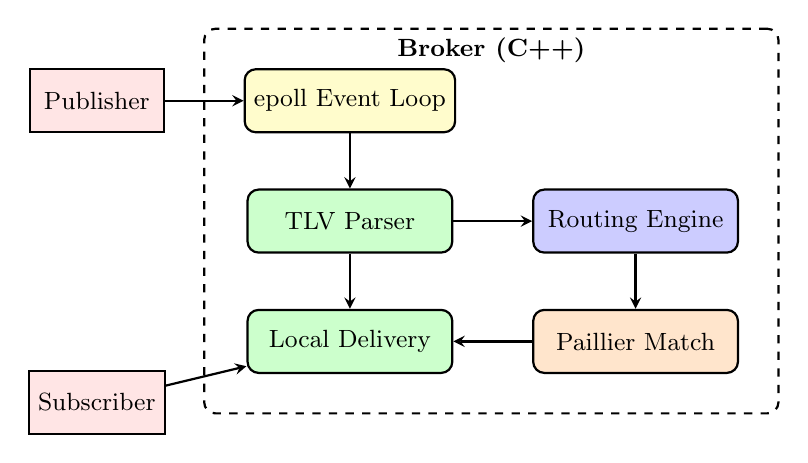
\begin{tikzpicture}[
    node distance=0.7cm and 1.0cm,
    box/.style={rectangle, draw=black, thick, rounded corners, minimum width=2.6cm, minimum height=0.8cm, text centered, font=\small},
    io/.style={rectangle, draw=black, thick, minimum width=1.7cm, minimum height=0.8cm, text centered, font=\small, fill=red!10},
    arrow/.style={->, >=stealth, thick}
]
\node (pub) [io] {Publisher};
\node (sub) [io, below=3.0cm of pub] {Subscriber};
\node (epoll) [box, right=of pub, fill=yellow!20] {epoll Event Loop};
\node (parser) [box, below=of epoll, fill=green!20] {TLV Parser};
\node (routing) [box, right=of parser, fill=blue!20] {Routing Engine};
\node (match) [box, below=of routing, fill=orange!20] {Paillier Match};
\node (delivery) [box, below=of parser, fill=green!20] {Local Delivery};
\draw [arrow] (pub) -- (epoll);
\draw [arrow] (sub) -- (delivery);
\draw [arrow] (epoll) -- (parser);
\draw [arrow] (parser) -- (routing);
\draw [arrow] (parser) -- (delivery);
\draw [arrow] (routing) -- (match);
\draw [arrow] (match) -- (delivery);
\node[draw, dashed, thick, rounded corners, fit=(epoll)(parser)(routing)(match)(delivery), inner sep=0.5cm, label={[anchor=north, font=\small\bfseries]north:Broker (C++)}] {};
\end{tikzpicture}%
}
\caption{DNS++ broker architecture. The epoll loop reads UDP datagrams, the zero-copy parser decodes TLV fields, and the routing engine consults the subscriber table IT\texttt{[]} and the neighbour table OT\texttt{[]}. The Match engine gates encrypted publications immediately before local delivery (Algorithm~\ref{alg:proximity}, lines 21--23).}
\label{fig:architecture}
\end{figure}

\subsection{Proximity Routing}

Algorithm~\ref{alg:proximity} sets out the publication path exactly as it is implemented. A subscriber that sends SUBSCRIBE is entered into the input table with \texttt{cached\_closest\_dist} initialised to infinity; when QUERY-MODE is set, the broker also returns the nearest publication already in cache on the spot, so a service that is up can be found immediately, with no waiting. Publications are always cached --- query-mode answers would otherwise not outlive later suppression --- and then pass through the brake on the upward path, the per-child quadrant cache, the local brake, the homomorphic Match gate, and finally the monotone filter applied to each subscriber. The cache is bounded at ten publications per routing key, evicted first-in-first-out, so query-mode answers reflect the ten most recent announcements rather than the full history.

That last filter is what gives ``Closest'' semantics: a subscriber is told about a replica only if it is strictly nearer than anything it already knows. Section~\ref{sec:dynamics} shows it is also the source of the system's principal dynamic limitation.

\begin{algorithm}[t]
\caption{Proximity Routing --- publication handling at a broker}
\label{alg:proximity}
\begin{algorithmic}[1]
\Require publication $p$ at $(lat_p, lon_p)$; routing key $k$; configuration $brakeScope$
\State $\textproc{CachePublication}(k, p)$ \Comment{unconditional, bounded FIFO: query-mode depends on it}
\If{$hasParent$ \textbf{and} $p$ not from parent}
    \If{$brakeScope \in \{\textit{upward}, \textit{both}\}$ \textbf{and not} $\textproc{BrakeAllows}(\textit{up}, k, lat_p, lon_p)$}
        \State $braked_{up}{+}{+}$ \Comment{brake active for this scope and it denies}
    \Else
        \State forward $p$ upward \Comment{brake inactive for this scope, or it allows}
    \EndIf
\EndIf
\ForAll{child brokers $c$ active for $k$}
    \If{$c$ is the origin of $p$}
        \State \textbf{continue} \Comment{avoid redundant echo; the monotone filter would deduplicate anyway}
    \EndIf
    \State $q \gets \textproc{QuadrantOf}(c.region, lat_p, lon_p)$; \; $d \gets dist(p, \textproc{QuadrantCentre}(c, q))$
    \If{$d < c.closestQuad[q]$} \Comment{information-aware filter}
        \State $c.closestQuad[q] \gets d$; forward $p$ down to $c$
    \EndIf
\EndFor
\State $S_k \gets$ subscribers in group $k$; \textbf{if} $S_k = \emptyset$ \textbf{then} \Return \Comment{local brake not charged}
\If{$brakeScope \in \{\textit{local}, \textit{both}\}$ \textbf{and not} $\textproc{BrakeAllows}(\textit{local}, k, lat_p, lon_p)$}
    \State $braked_{local}{+}{+}$; \Return
\EndIf
\If{$heEnabled$ \textbf{and} $p$ carries $bval_n$} \Comment{one Match per \emph{group}, not per subscriber}
    \State $s_0 \gets$ first element of $S_k$; \textbf{if not} $\textproc{ExecuteMatch}(bval_n, s_0.bval_{m1}, s_0.bval_{m2})$ \textbf{then} \Return
\EndIf
\ForAll{$s \in S_k$}
    \State \textbf{if} $dist(p, s) < s.cachedClosestDist$ \textbf{then} deliver $p$ to $s$; \; $s.cachedClosestDist \gets dist(p, s)$
\EndFor
\end{algorithmic}
\end{algorithm}

\textbf{Propagation brake.} The brake limits how many publications a broker propagates from one spatial quadrant within a sliding window. Each quadrant maintains a timestamp queue; a publication propagates only when fewer than \texttt{brake\_limit} entries arrive within \texttt{brake\_window} seconds. A \texttt{brake\_scope} parameter (\texttt{upward}, \texttt{local}, \texttt{both}; default \texttt{both}) governs which directions are gated, each with its own window so that one direction does not consume the other's quota. The distinction is material: under \texttt{upward} the brake has no effect at all on a single broker, which has no parent. When \texttt{brake\_scope} excludes a direction, publications along that path are propagated unconditionally rather than suppressed by default; the brake is strictly opt-in per direction. This nuance is worth noting because an earlier revision of this implementation gated solely the upward path, quietly rendering the single-broker brake sweep vacuous.

Two orderings matter later. The empty-group test precedes the local brake, so $braked_{local}$ is charged only for publications that had somewhere to go; and the Match gate follows the brake, so a braked publication never reaches the cryptographic path (Section~\ref{sec:crypto}).

\textbf{Distance.} We use the equirectangular approximation $d = \sqrt{\Delta\text{lat}^2 + (\Delta\text{lon}\cos\bar{\text{lat}})^2}$ about the mean latitude of the two points, sufficient for \emph{ranking} candidates and avoiding Haversine's trigonometric cost on the hot path. Section~\ref{sec:limitations} notes where it departs from true distance.

\subsection{Hierarchical Overlay}
\label{sec:overlay}

Each broker reads identifier, listen port, parent address, coordinates and brake parameters from a configuration file (Appendix~\ref{app:config}). Children send HELLO on startup, registering coordinates; the parent computes its Minimum Bounding Hyperrectangle (MBH) as the union of its children's regions. A leaf receiving a local subscription propagates it upward, and the parent records which children are active for that name in OT\texttt{[]}. Publications then flow in three directions: upward subject to the brake, downward subject to quadrant filtering, and locally subject to the brake, the Match gate and then the monotone filter. Leaves update their MBH as clients register and propagate changes upward via REGION\_UPDATE, so parents make quadrant decisions against accurate coverage.

\subsection{Privacy-Preserving Matching}
\label{sec:privacy}

\textbf{Threat model.} We assume an \emph{honest-but-curious} broker: it executes the protocol faithfully but may record everything it observes and attempt to infer which service a given subscriber is interested in. The design goal is that a broker learn neither the subscribed name nor the published name, only whether a publication matches a subscription group. Endpoints are trusted with their own key material; brokers are assumed not to collude with the HEPS. Network adversaries are explicitly out of scope, since the prototype carries neither transport security nor message authentication (Section~\ref{sec:limitations}). Section~\ref{sec:limitations} states precisely which parts of this goal the implementation meets and which it does not.

Subscriptions and publications carry blinded values rather than names. We implement the modified Paillier cryptosystem of \citet{rio2026dnspplus}, following the protocols of \citet{nabeel2012efficient}. A Homomorphic Encryption Parameter Service (HEPS) generates a 2048-bit key pair; the private key $\lambda$ blinds, while $(n, g, \mu)$ suffices for the unblinding brokers perform. Throughout, the subscript $n$ marks the \emph{notification} (publisher) side of a blinded value and $m$ the \emph{matching} (subscriber) side; $n$ standing alone always denotes the Paillier modulus. Three mechanisms underpin the protocol. \emph{Blinding cancellation}: the HEPS issues $(e_m, d_m)$ with $d_m = n - e_m$, and since $g = 1+n$ has order exactly $n$ in $(\mathbb{Z}/n^2\mathbb{Z})^*$, $g^{e_m}g^{d_m} = g^n \equiv 1$. \emph{Randomness stripping}: raising a ciphertext to the $\lambda$-th power eliminates its randomness, as $r^{n\lambda} \equiv 1 \pmod{n^2}$ by Carmichael's theorem. \emph{Value-domain separation}: a fixed stretching factor $r_m$ and per-execution random $r$ place positive differences in $[0, n/2)$ and negative ones in $(n/2, n)$.

\begin{lemma}
\label{lem:match}
Let $bval_n(x) = g^{e_m} g^{\lambda(r_m x + r)} \bmod n^2$ and $bval_m(-v) = g^{d_m} E(-v)^{r_m \lambda} \bmod n^2$, with $e_m + d_m \equiv 0 \pmod{\mathrm{ord}(g)}$ and $g = 1+n$. Then $L\big(bval_n(x) \cdot bval_m(-v) \bmod n^2\big) \cdot \mu \equiv r_m(x - v) + r \pmod{n}$.
\end{lemma}
\begin{corollary}[Correctness of the threshold test]
\label{cor:threshold}
With $0 < r < r_m$ and $r_m|x-v|_{\max} + r < n/2$, we have $\textit{diff} < n/2 \iff x \ge v$.
\end{corollary}

Equality is decided by two invocations --- verifying $x \ge v$ against $bval_m(-v)$ and $x < v+1$ against $bval_m(-(v+1))$ --- and a match declared only if both hold. The broker learns the two Boolean outcomes; note, however, that the recovered magnitude $\textit{diff}$ encodes $r_m(x-v)+r$, so a party holding $r_m$ can extract ordering information about hashed names even without $\lambda$.

\textbf{Subscription grouping and its cost.}
Blinded values are semantically secure, so a ciphertext cannot serve as a lookup key: indexing by $bval$ would put every subscriber in a group of one and force one Match per subscriber per publication.
This implementation instead hashes the plaintext service name and groups on that hash, restoring one-Match-per-group batching (Algorithm~\ref{alg:proximity}, line~22).
Only the ingress broker sees the plaintext name; inter-broker forwarding carries the 64-bit digest, which is unkeyed and enumerable and so is not protection by itself (Section~\ref{sec:limitations}).
The homomorphic Match accordingly re-checks a decision already taken on the hash rather than determining routing --- a deliberate trade-off quantified in Section~\ref{sec:limitations}.
The Cover protocol of \citet{nabeel2012efficient} aggregates subscriptions without exposing them and remains future work.

\section{Implementation}
\label{sec:impl}

The system is C++17 built with CMake. Level-triggered epoll suits datagram semantics because each \texttt{recvfrom()} returns one complete message and readiness persists while data remains. The epoll timeout doubles as the TTL garbage-collection timer, avoiding extra descriptors. Parsing is zero-copy. The buffer is reinterpreted as the fixed header and traversed by pointer arithmetic, with length validation before each access. Socket descriptors follow RAII, and a dedicated logger thread drains a producer--consumer queue so that log I/O never blocks the event loop.

The Paillier layer is built over GMP. Key generation forces the top two bits of each prime factor, guaranteeing a modulus of exactly the requested width; without this, $p \cdot q$ can fall short, and we observed moduli between 2040 and 2048 bits before the fix. The random state is seeded once per instance rather than per operation, the previous per-call reseeding having invoked \texttt{std::random\_device} on every encryption and materially inflated measured cryptographic cost. Expensive exponentiations are confined to publishers and subscribers; brokers execute only modular multiplications and $L(\cdot)$.

\textbf{Observability.} Because a silent fallback to plaintext would be indistinguishable from a successful encrypted run, brokers export twelve counters (\texttt{STATS\_DATA\_EXT}), including Match invocations and hits, publications suppressed in each direction, subscription-group count, and whether homomorphic matching is active. Every encrypted result in Section~\ref{sec:eval} is accompanied by a non-zero Match count. Key loading fails fast unless a flag explicitly permits plaintext fallback, and any fallback is announced at startup.

\section{Evaluation}
\label{sec:eval}

\subsection{Setup}

Experiments ran on Ubuntu Linux, kernel 7.0.0-30-generic, on an AMD Ryzen~9 8945HS with two cores available to the virtual machine, GMP 6.3.0, GCC 13.3.0, CMake \texttt{Release}. Publishers and subscribers are benchmark clients placed uniformly at random over latitude $[-90,90]$ and longitude $[-180,180]$. We measure \textbf{recall} (proportion of subscribers receiving their true nearest publisher), \textbf{stretch} (received distance divided by ground-truth nearest, optimal 1.0), \textbf{traffic ratio} (total forwarding events over successful local deliveries), and \textbf{convergence time} after a migration. An effectively unbounded brake serves as the internal baseline; we implement it as \texttt{brake\_limit}=1000, at which the measured suppression rate is exactly zero, and label it $\infty$ in figures. Plaintext matching is the baseline for the cryptographic evaluation.

Each configuration was repeated for 30 independent trials, each with its own derived seed, so trials are independent samples rather than repetitions of one placement. Three warm-up trials precede every measured run and are discarded. We report means with 95\% bootstrap confidence intervals (10{,}000 resamples, percentile method), appropriate here because recall and stretch are bounded and symmetric standard-deviation bars would extend past those bounds. The plaintext--encrypted comparison uses a paired Wilcoxon signed-rank test. Recall and stretch are deterministic functions of the trial seed, so a configuration re-measured under an unchanged seed sequence reproduces the same values; this is why the \texttt{brake\_limit}=4 row recurs identically across Tables~\ref{tab:brake-sweep}, \ref{tab:scale} and \ref{tab:crypto-comparison}.

\subsection{Single-Broker Brake Sweep}
\label{sec:single-brake}

We sweep \texttt{brake\_limit} over $\{1,2,4,1000\}$ with 10 publishers and 50 subscribers and \texttt{brake\_scope=both}; with no parent, only the local arm is active. Table~\ref{tab:brake-sweep} reports recall and stretch with the \emph{measured} suppression rate, read from the \texttt{braked\_local} counter rather than inferred from recall; Figure~\ref{fig:single-brake-app} plots the same data with confidence intervals.

\begin{table}[t]
\centering
\caption{Single-broker brake sweep (10 publishers, 50 subscribers, 30 trials). Suppression is $\textit{braked\_local}/\textit{pub\_received}$. Brackets are 95\% bootstrap CIs.}
\label{tab:brake-sweep}
\begin{tabular}{lccc}
\toprule
Brake limit & Recall & Stretch & Suppression \\
\midrule
1    & 0.452 [0.405, 0.499] & 2.172 [1.970, 2.385] & 0.624 \\
2    & 0.749 [0.699, 0.797] & 1.373 [1.261, 1.497] & 0.321 \\
4    & 0.983 [0.965, 0.996] & 1.013 [1.001, 1.030] & 0.033 \\
1000 & 1.000 [1.000, 1.000] & 1.000 [1.000, 1.000] & 0.000 \\
\bottomrule
\end{tabular}

\vspace{3pt}
\parbox{0.93\textwidth}{\footnotesize The broker's counters are cumulative over process lifetime and therefore span 330 publications --- the 300 of the measured trials plus the 30 of the three discarded warm-up trials --- whereas recall and stretch are computed over measured trials only. Warm-up and measured trials draw from the same placement distribution, so the suppression rate is unaffected to three decimal places.}
\end{table}

The brake behaves as designed, and the trade-off is steep. At \texttt{brake\_limit}=1 the broker suppresses 62.4\% of publications (206 of 330) and recall falls to 0.452, with surviving subscribers reaching replicas 2.17$\times$ farther than optimal on average. At 4, suppression is 3.3\% and recall recovers to 0.983 at near-optimal stretch. With the brake disabled, recall and stretch are exactly 1.000, confirming Algorithm~\ref{alg:proximity} correct in the absence of throttling. The stretch distributions (Figure~\ref{fig:stretch-cdf}) show that tightening the brake leaves most subscribers at their optimum while displacing a minority a long way.

Recall consistently exceeds $1 - \textit{suppression}$ --- 0.452 against 0.376 at limit 1, 0.983 against 0.967 at limit 4. The gap is not noise: it reflects publications suppressed that would not have been anyone's nearest replica. Suppression costs recall only when the suppressed publication was someone's optimum, and under uniform placement most are not.

\subsection{Multi-Broker Hierarchical Routing}
\label{sec:multi-brake}

We extend to a three-broker tree --- one root, two leaves at London and Berlin --- with 20 publishers and 50 subscribers attached to their nearest leaf, so both arms of the brake are active. Table~\ref{tab:multi-broker} reports the sweep; Figure~\ref{fig:multi-broker} plots it.

\begin{table}[t]
\centering
\caption{Multi-broker brake sweep (three-broker tree, 20 publishers, 50 subscribers, 30 trials).}
\label{tab:multi-broker}
\begin{tabular}{lccc}
\toprule
Brake limit & Recall & Stretch & Traffic ratio \\
\midrule
1    & 0.227 [0.201, 0.253] & 3.331 [3.038, 3.640] & 1.087 [1.082, 1.092] \\
2    & 0.458 [0.424, 0.493] & 2.086 [1.885, 2.301] & 1.109 [1.104, 1.115] \\
4    & 0.779 [0.751, 0.805] & 1.318 [1.237, 1.409] & 1.142 [1.136, 1.148] \\
1000 & 0.981 [0.966, 0.992] & 1.013 [1.003, 1.027] & 1.168 [1.162, 1.174] \\
\bottomrule
\end{tabular}
\end{table}

\textbf{The brake is a bad deal in a two-level tree.} Tightening the limit from 1000 to 1 lowers the traffic ratio from 1.168 to 1.087, a 6.9\% reduction in forwarding events. But recall drops from 0.981 to 0.227, and stretch climbs from 1.013 to 3.331. At the most aggressive setting we throw away roughly three quarters of correct resolutions to save 7\% of traffic. Even \texttt{brake\_limit}=4 costs 20 points of recall for a 2.2\% saving.

\textbf{The quadrant cache does the useful filtering.} With the brake off, the traffic ratio is already only 1.168, so each delivery costs 0.168 extra forwarding events. That floor is set by the downward quadrant cache, which forwards to a child only what would improve that child's closest distance for the quadrant. The brake moves another 0.081 below this floor, but it gets there by dropping events at a fixed rate, not by removing redundant work.

% 已核实 (results/final/multi_brake_1.log)：15/17 是「三 broker 之和」且是「单个 trial」的值，
% 不是 30-trial 累计。benchmark 只打印求和后的计数器，leaf1/leaf2 无法拆分，故改用聚合口径 +
% 拓扑论证说明 root 贡献为零。分母改为「每个 trial 原发的 20 条 publication」，而非 pub_received。
\textbf{Braking compounds across levels.} At the same limit, recall in the tree is worse than in the single broker, 0.227 against 0.452 at limit 1. A publication must survive three independent gates --- the ingress leaf's upward brake, the root's quadrant-cache forwarding decision, and the destination leaf's local brake --- so the suppression probabilities multiply rather than add. The counters bear this out. In a representative trial at \texttt{brake\_limit}=1 the tree recorded 15 upward-suppressed and 17 locally-suppressed publications summed over all three brokers, against the 20 a trial originates: more than one suppression event per publication issued. The root contributes to neither total and by construction cannot, having no parent and no local subscribers, so the two symmetric leaves account for both. These are per-trial figures, not cumulative; across trials each direction varied between roughly 15 and 18. The harness sums these counters across brokers before recording them, so we report the aggregate rather than a per-leaf split.

\textbf{Comparison with the original simulation.} The trends agree --- recall falls and stretch rises as the brake tightens --- but the magnitude does not, and two differences probably explain why. At our scale, 20 publishers over four global quadrants give roughly five publications per quadrant per window, so a limit of 1 or 2 binds almost immediately, whereas at simulation scale ($10^6$ publishers) the same limit is a far smaller fraction of offered load. And uniform placement produces no clustering, whereas population-weighted placement concentrates publishers where subscribers are, making a suppressed publication more likely to have a near-equivalent substitute. Both predict that an \emph{absolute} brake count becomes progressively more aggressive as density falls (Section~\ref{sec:brake-discussion}).

\subsection{Scalability}
\label{sec:scale}

Fixing \texttt{brake\_limit}=4 and 10 publishers, we vary subscribers from 10 to 1000, sampling kernel UDP statistics from \texttt{/proc/net/snmp} before and after each run (Table~\ref{tab:scale}, Figures~\ref{fig:udp-loss} and~\ref{fig:scale-app}). The 50-subscriber row therefore repeats the \texttt{brake\_limit}=4 configuration of Table~\ref{tab:brake-sweep}, and is reproduced here for continuity.

\begin{table}[t]
\centering
\caption{Subscriber-count scaling (\texttt{brake\_limit}=4, 10 publishers, 30 trials). UDP errors are the measured delta in \texttt{RcvbufErrors}.}
\label{tab:scale}
\begin{tabular}{lccc}
\toprule
Subscribers & Recall & Stretch & UDP \texttt{RcvbufErrors} \\
\midrule
10   & 0.983 [0.953, 1.000] & 1.007 [1.000, 1.021] & 0 \\
50   & 0.983 [0.965, 0.996] & 1.013 [1.001, 1.030] & 0 \\
200  & 0.982 [0.966, 0.995] & 1.014 [1.004, 1.026] & 0 \\
500  & 0.879 [0.811, 0.939] & 1.017 [1.005, 1.033] & 1818 \\
1000 & 0.833 [0.747, 0.904] & 1.017 [1.005, 1.031] & 4963 \\
\bottomrule
\end{tabular}
\end{table}

Up to 200 subscribers recall holds at 0.98 with stretch within 1.5\% of optimal and zero overflows. Beyond that, recall degrades to 0.879 and 0.833 while overflows rise to 1818 and 4963. The correlation alone would only suggest a cause; the stretch column identifies the mechanism. \emph{Stretch does not degrade where recall does}: the 1.017 measured at 500 and 1000 subscribers is indistinguishable from the 1.014 at 200, with overlapping intervals throughout. Had routing been failing to identify nearest replicas, subscribers would have been steered to worse ones and stretch would have risen. Instead, subscribers that receive a publication still receive the optimal one; the losses are datagrams the kernel discarded when hundreds of sockets are polled from one process on a two-core host. This is a limitation of the harness, not the algorithm, and precisely the class of effect a discrete-event simulation cannot exhibit. Enlarging \texttt{SO\_RCVBUF} to 4\,MiB (the kernel granted 8) did not eliminate it, indicating the bottleneck is the single-threaded polling loop rather than buffer capacity.

\subsection{Privacy Layer Overhead}
\label{sec:crypto}

We measured one workload twice under identical conditions: a single broker with 10 publishers and 50 subscribers at \texttt{brake\_limit}=4, run 30 times in plaintext mode and 30 times with 2048-bit encrypted matching, the two arms paired by seed and executed back to back. Endpoint blinding was completed before the timing window opened, so the measurement isolates broker-side cost. Table~\ref{tab:crypto-comparison} reports the outcome and Figure~\ref{fig:crypto-app} the per-trial distributions.

\begin{table}[t]
\centering
\caption{Plaintext versus encrypted matching (30 paired trials). See the caveat on absolute latency below.}
\label{tab:crypto-comparison}
\begin{tabular}{lcccc}
\toprule
Mode & Recall & Stretch & Latency mean (ms) & Median (ms) \\
\midrule
Plaintext & 0.983 [0.965, 0.996] & 1.013 [1.001, 1.030] & 63.6 [60.3, 67.2] & 62.6 \\
Encrypted & 0.983 [0.965, 0.996] & 1.013 [1.001, 1.030] & 63.4 [60.5, 66.4] & 63.0 \\
\bottomrule
\end{tabular}
\end{table}

Taking the paired difference as \emph{encrypted minus plaintext} throughout, a Wilcoxon signed-rank test over the 30 pairs returns $W = 182$ (the smaller of the two signed-rank sums), $z = -1.04$ and $p = 0.299$. The median paired difference is $+0.377$\,ms with a 95\% bootstrap confidence interval of $[-0.310, +1.051]$\,ms (10{,}000 resamples, percentile method); the mean paired difference is $-0.174$\,ms, of opposite sign, which is itself an indication that the two arms are not separated. We therefore cannot reject the hypothesis that the two modes have the same per-publication latency. We do not claim they are equivalent: what makes this result informative rather than merely negative is the resolution of the experiment, which we quantify below alongside the bound.

\textbf{The encrypted arm was verifiably encrypted.} A silent fallback to plaintext would have produced exactly these numbers, so the counters settle it: 319 \texttt{executeMatch} invocations in the encrypted runs and none in plaintext. That figure is itself consistent with the rest of the measurement --- the Match gate sits after the local brake, so of the 330 publications the broker received it should see the 96.7\% the brake admitted, or 319. Recall and stretch matched to three decimal places across the two arms, so the gate admitted every publication that plaintext routing delivered and rejected none: the re-check never altered an outcome, as expected when the routing decision is taken before the Match runs (Section~\ref{sec:privacy}).

\textbf{We bound the broker-side cost rather than argue from a null result.} Absence of a detectable difference is weak evidence alone. Appendix~\ref{app:microbench} measures a single Match at 0.0127\,ms (Table~\ref{tab:microbench}). A broker performs one Match per subscriber \emph{group} per publication, so with $S$ groups the added cost per publication is bounded by $S \times 0.0127$\,ms. The group count reported by the counters is a snapshot taken after the run, once TTL expiry has retired inactive entries, and is therefore not a safe upper bound on $S$ during the run. We instead take the counterfactual worst case in which grouping fails entirely and each of the 50 subscribers forms its own group --- a configuration this implementation cannot actually enter, since hashing is what restores grouping, but one that bounds any implementation that indexed by ciphertext --- giving $50 \times 0.0127 = 0.635$\,ms. Even this pessimistic bound is under 1\% of the measured per-publication latency, and it lies below what the paired experiment was capable of resolving. The 30 paired differences have a sample standard deviation of 4.37\,ms; at $\alpha = 0.05$ two-sided and 80\% power, 30 pairs detect a paired difference of 2.23\,ms or larger (2.31\,ms using exact $t$ quantiles at 29 degrees of freedom). The pessimistic bound of 0.635\,ms is less than a third of that minimum detectable effect. The null result is therefore precisely what the micro-benchmark predicts --- not evidence that the privacy layer is free, but evidence that its broker-side cost is smaller than this experiment was built to see, with the micro-benchmark supplying the number the end-to-end measurement cannot. It also extrapolates: cost grows linearly in \emph{distinct subscription groups}, not in subscribers or publications, so $10^4$ concurrent groups would add roughly 127\,ms of broker CPU per publication.

\textbf{The cost lives at the endpoints.} Blinding a notification costs 23.47\,ms and a subscription 58.97\,ms --- 1848$\times$ and 4643$\times$ a broker-side Match (Figure~\ref{fig:crypto-breakdown}). Both are one-off, off the routing path: a publisher blinds once per announcement, a subscriber once per subscription, and the result is reused for every subsequent match. This is the workload partition DNS++ intends, and it holds on real hardware.

\begin{figure}[t]
\centering

\includegraphics[width=0.62\textwidth]{fig_crypto_breakdown.png}
\caption{Cost decomposition of the privacy layer, logarithmic scale. Endpoint blinding dominates by more than three orders of magnitude.}
\label{fig:crypto-breakdown}
\end{figure}

\textbf{Caveat on absolute latency.} These values are not throughput figures: the harness dispatches all publications before polling subscriber sockets, and on two cores the inter-publication sleep overshoots substantially, so absolute latency varies between runs by an order of magnitude. The paired design --- identical seeds and placement, back to back --- cancels that noise, so we report only the comparison.

\subsection{Dynamics: Convergence After Replica Migration}
\label{sec:dynamics}

The central hypothesis holds that DNS++ propagates service changes in seconds rather than the minutes-to-hours of TTL expiry. On a single broker with plaintext matching, with 20 publishers and 50 subscribers on one service, we let the system settle, then perform 20 migrations per trial: move a random publisher to a new random location and re-publish, recording for every subscriber whose correct nearest replica changes the time until it receives that replica, with a 1\,s timeout. All runs are brake-free, verified by the \texttt{braked} counter reading zero --- a throttled publication would otherwise be indistinguishable from a failure to converge. Migrations fall into two classes under the monotone filter: \textbf{closer}, where the migrated replica lands nearer than the subscriber's cached distance and is admitted; and \textbf{farther}, where the subscriber's own replica moved away and its optimum is now a \emph{different} replica. Table~\ref{tab:dynamics} summarises both classes and Figure~\ref{fig:dynamics-cdf} gives the full closer-class distribution.

\begin{table}[t]
\centering
\caption{Replica migration convergence: single broker, plaintext matching, brake-free (20 publishers, 50 subscribers, 20 migrations per trial, 30 trials). \emph{Events} counts subscriber--migration pairs whose correct nearest replica changed.}
\label{tab:dynamics}
\begin{tabular}{lcccc}
\toprule
Migration class & Events & Converged & Median (ms) & p95 (ms) \\
\midrule
closer  & 1036 & 998 (96.3\%) & 0.42 & 1.24 \\
farther & 1391 & 0 (0.0\%)    & ---  & ---  \\
\bottomrule
\end{tabular}
\end{table}

Closer-class migrations converge in a median of 0.42\,ms, 95th percentile 1.24\,ms --- against a typical 300\,s TTL, roughly five orders of magnitude faster, and comfortably inside the ``seconds, not minutes'' target. The 3.7\% that did not converge are a second-order effect of the same filter. A subscriber's cached distance is set by the replica that was closest when the cache was filled. If that replica later moves away, the subscriber keeps the stale minimum, and even a genuinely closer replica can be rejected.

Farther-class migrations never converge: zero of 1391. This is not an implementation defect; it follows directly from the design. Updates are push-only and gated on strict improvement. Once a subscriber's replica has moved away, a better alternative can reach the subscriber only if it re-publishes \emph{and} is strictly closer than the now-stale cached distance. Neither condition is guaranteed, and neither occurred.

We repeated the experiment with encrypted matching under the same seed. Placement is seed-determined, so the closer class holds the identical 1036 events and the farther class 1397 rather than 1391, six events differing through delivery timing rather than any routing decision. We report the plaintext run throughout, and record the repetition here so its absence is not read as an untested case.

The dynamics claim therefore needs a direction. DNS++ converges sub-millisecond when a service moves \emph{closer} or a new replica appears. When a service moves \emph{away} or disappears, it does not converge at all. Affected subscribers keep stale state until a closer publication arrives or the subscription expires.

\section{Discussion}
\label{sec:discussion}

\subsection{The Brake Trade-off, and Why the Quadrant Cache Wins}
\label{sec:brake-discussion}

Our measurements turn an inference into an observation. Suppression costs recall only when the suppressed publication was someone's optimum, which is why recall exceeds $1 - \textit{suppression}$ throughout; in the three-broker tree the trade is nonetheless 6.9\% of forwarding events saved for 77\% of correct resolutions lost.

The brake is therefore better read not as an efficiency knob but as an overload valve: a way to keep a broker functioning under publication storms, at a recall cost severe enough that it should not engage in normal operation. It follows that any sensible setting must scale with publisher density. In our 20-publisher tree over four quadrants, a limit of 4 already suppresses a quarter of publications, so a deployment with thousands of replicas per quadrant would need a proportionally higher limit. An absolute count is the wrong unit; a limit expressed as a fraction of observed quadrant load over the preceding window would degrade gracefully instead of tightening silently as density falls.

The deeper point is selectivity. DNS++ contains two traffic-reduction mechanisms, and they are not equivalent. The quadrant cache is \emph{information-aware}: it suppresses a publication precisely when a better one has already been forwarded for that region, so suppression is nearly free in recall terms. Alone it reaches a traffic ratio of 1.168 at 0.981 recall, close to the floor a tree topology permits. The brake is \emph{rate-based}: it counts events in a window and drops the excess, with no notion of whether what it drops was anyone's optimum. The first is a filter; the second is a fuse.

In a two-level tree the cache suffices alone, and the brake should sit high enough never to engage. Its value is as a safety mechanism, and potentially in deeper hierarchies where upward traffic accumulates, a regime our topology cannot exercise. An information-aware \emph{upward} filter, applying quadrant-cache logic to the parent direction, would likely dominate the brake on both axes.

\subsection{Privacy, Performance, and What the Measurement Establishes}

The privacy layer's cost is dominated by endpoint blinding, not broker routing. Once blinding is amortised, the broker adds at most $S \times 0.0127$\,ms per publication, under 0.635\,ms even on the pessimistic assumption that grouping fails entirely at the scale measured. This is the intended DNS++ workload partition, and it holds on real hardware: expensive exponentiations sit with publishers and subscribers, which perform them infrequently and independently, while the routing infrastructure stays fast.

\textbf{What the bound implies for a deployment.} Because cost is linear in \emph{distinct subscription groups} and independent of subscriber count, the capacity question a deployer faces is not ``how many clients?'' but ``how many distinct services?''. A broker serving $10^6$ subscribers spread over $10^3$ services costs the same per publication as one serving $10^3$ subscribers over the same $10^3$ services: roughly 12.7\,ms of CPU, or some 79 publications per second per core. At $10^4$ groups the same arithmetic gives 127\,ms and about 8 publications per second --- a figure low enough that the sharding key for a production overlay must be the service namespace, not the client population or the geographic region. This is a direct and testable consequence of the measured Match cost, and it is the opposite of the intuition that a privacy-preserving resolver scales badly in users.

One qualification on what the measurement establishes: as implemented, the ingress broker also sees the plaintext service name. The result therefore shows that homomorphic matching \emph{can} be made cheap on a name-resolution critical path; it does not by itself show that this implementation provides privacy. For latency-critical deployments, blinding could be reduced by smaller keys (trading security), GPU acceleration \citep[which reports 9.6M matches per second on an H100]{rio2026dnspplus}, or caching blinded values for repeated names, none of which requires broker changes.

\subsection{Limitations}
\label{sec:limitations}

\paragraph{Privacy as implemented.} Our brokers index routing tables by a hash of the plaintext service name rather than by ciphertext, because blinded values are semantically secure and cannot serve as lookup keys without destroying grouping (Section~\ref{sec:privacy}). The ingress broker therefore learns the name; upstream brokers see only the 64-bit digest, which narrows but does not close the exposure, since the digest is unkeyed and the name space is small enough to enumerate. The homomorphic Match is a formal re-check rather than the routing mechanism --- \emph{this is the configuration under which Section~\ref{sec:crypto}'s figures were obtained}. The hash is neither keyed nor collision-resistant: at a DNS-scale space of $\approx 2^{30}$ names its 64-bit output gives a collision probability near 3\%. A collision has two consequences, and the second is the more serious. Distinct names are placed in one group, so a publication for one can be delivered to subscribers of the other; and because the Match gate is evaluated once against the group representative (Algorithm~\ref{alg:proximity}, line~22), a representative belonging to the colliding name causes the gate to reject the publication for the \emph{entire} group, denying delivery even to subscribers whose name genuinely matched. A keyed, fixed-width hash with an explicit collision policy --- per-group verification rather than representative verification --- would remove the second failure mode without restoring grouping cost. Separately, the prototype co-locates HEPS with the root broker, which retains $\lambda$, $e_m$, $d_m$ and $r_m$; a party holding these can blind candidate names and match them against stored subscriptions, mounting a dictionary attack over a space whose entropy is far below 2048 bits. And the recovered magnitude leaks ordering information to any holder of $r_m$. Against the honest-but-curious broker of Section~\ref{sec:privacy}, we therefore make no claim of deployment-grade privacy. Decoupling routing keys from ciphertext via the Cover protocol \citep{nabeel2012efficient}, and separating HEPS from the broker, are the principled fixes.

\paragraph{One-directional convergence.} The monotone filter gives sub-millisecond convergence when replicas move closer and none at all when a subscriber's replica moves away (Section~\ref{sec:dynamics}). Closing this requires soft state or an explicit invalidation path, neither present in the current design.

\paragraph{Measurement methodology.} Our harness dispatches all publications for a trial before polling sockets, and the inter-publication sleep overshoots on two cores: the same configuration differed by an order of magnitude in absolute latency between driver runs, so we report latency only for the paired comparison. Beyond 200 subscribers, recall degrades because a single-threaded client cannot drain hundreds of sockets fast enough and the kernel drops datagrams; stretch does not degrade there, confirming routing remains correct for delivered publications. Both ceilings are in the harness, not the broker.

\paragraph{Implementation shortcuts.} The equirectangular distance does not wrap at the antimeridian, so pairs spanning $\pm 180^\circ$ appear nearly a full circumference apart. Uniform lat/lon sampling also over-samples the poles, where the approximation is weakest. Ground truth and broker use the \emph{same} function, so internal consistency of recall and stretch is unaffected; only fidelity to geodesic distance is.

The routing key is derived with \texttt{std::hash<std::string>}, whose value is implementation-defined; reproducing our routing decisions bit-for-bit therefore depends on the standard-library version as well as the seed, and a deployment would want a specified hash such as SipHash instead. Exponentiations with secret exponents use \texttt{mpz\_powm} rather than the constant-time variant, leaving a timing side channel. The protocol carries no authenticator, so any host that reaches a broker can forge HELLO, REGION\_UPDATE, or PUBLISH and corrupt MBH aggregation. The relationship between the hash width $l$ and the stretching factor $r_m$ is intended to be derived rather than independently fixed; it drifted out of sync when the hash implementation changed (Appendix~\ref{app:microbench}).

\paragraph{Scope.} All processes run on loopback with no emulated delay or loss, so latency figures isolate protocol and CPU cost and should not be read as wide-area performance. The multi-broker evaluation uses a three-broker, two-level tree; deeper hierarchies are unmeasured, and the brake is expected to matter more there. Placement is uniformly random rather than population-weighted, limiting comparability with the original simulation, and the evaluated scale remains orders of magnitude below its $10^6$ endpoints. Finally, although our hypothesis is framed relative to conventional DNS, we do not measure a production resolver under matched conditions; the brake-unbounded configuration is an internal baseline only.

\section{Conclusion}
\label{sec:conclusion}

We have presented the first real-system implementation of the DNS++ broker architecture --- Algorithm~\ref{alg:proximity}, a multi-broker overlay with dynamic MBH aggregation, and the modified Paillier privacy layer --- together with a reproducible measurement harness.

Three results emerge. The propagation brake is blunter than simulation suggested: in a three-broker tree it buys a 6.9\% reduction in forwarding events at the cost of 77\% of correct resolutions, whereas the quadrant cache alone attains a traffic ratio of 1.168 at 0.981 recall. The distinction is selectivity --- the cache suppresses what is redundant, the brake what exceeds a rate --- which argues for treating the brake as an overload valve rather than an efficiency parameter. On the broker side, the privacy layer costs at most $S \times 0.0127$\,ms in the number of subscription groups $S$: three orders of magnitude below endpoint blinding, and below what a paired 30-trial comparison could resolve ($p = 0.299$, minimum detectable effect 2.23\,ms). Because that cost is linear in services and flat in clients, the sharding key for a deployment is the namespace, not the client population. Convergence after migration is likewise directional: sub-millisecond when a replica moves closer, absent when it moves away.

We are explicit that the implementation does not deliver the privacy the design intends: restoring subscription grouping under semantically secure ciphertexts required indexing on a hash of the plaintext name, so the ingress broker learns what it was meant not to. What we establish is that the homomorphic machinery is cheap enough to sit on a name-resolution critical path --- a necessary condition for the design, not a sufficient one. Future work follows directly: an information-aware upward filter to replace the rate-based brake; the Cover protocol to recover the intended privacy property; soft state to make convergence bidirectional; a HEPS separated from the broker; and a harness able to exercise deeper hierarchies and larger endpoint counts.

\bibliographystyle{tmlr}
\bibliography{main}

\newpage
\appendix

\section{Requirement Coverage}
\label{app:gap}

\begin{table}[H]
\centering
\caption{Coverage of the three requirements. $\bullet$ = addressed, $\circ$ = partially addressed, blank = not addressed.}
\small
\begin{tabular}{p{0.54\textwidth}ccc}
\toprule
System class & Privacy & Dynamics & Locality \\
\midrule
DoT / DoH / DoQ \citep{hu2016dot,hoffman2018doh,huitema2022doq} & $\circ$ & & \\
Oblivious DNS / DoH \citep{schmitt2019odoh,singanamalla2021odoh} & $\bullet$ & & \\
PIR-based DNS \citep{bhat2019pir,papadopoulos2020pir}           & $\bullet$ & & \\
EDNS Client Subnet \citep{contavalli2016ecs}                    & & & $\bullet$ \\
Anycast / CDN routing \citep{calder2015anycast}                 & & $\circ$ & $\circ$ \\
Spatial pub/sub \citep{gupta2004meghdoot,castro2002scribe}      & & $\bullet$ & $\bullet$ \\
Privacy-preserving pub/sub \citep{nabeel2012efficient}          & $\bullet$ & $\bullet$ & \\
\midrule
DNS++ \citep{rio2026dnspplus}                                   & $\bullet$ & $\bullet$ & $\bullet$ \\
\bottomrule
\end{tabular}
\end{table}

\section{TLV Protocol Specification}
\label{app:tlv}

The fixed 8-byte header carries \texttt{msg\_type} (uint16), \texttt{num\_tlvs} (uint16) and \texttt{payload\_len} (uint32).

\begin{table}[H]
\centering
\caption{TLV field type definitions.}
\label{tab:tlv}
\begin{tabular}{lll}
\toprule
Type name & Code & Size \\
\midrule
COORDINATES & 0x0001 & 8 bytes (float lat, float lon) \\
FLAGS & 0x0002 & 4 bytes (uint32\_t bitmask) \\
SERVICE\_NAME & 0x0003 & Variable (UTF-8 string) \\
BRAKE\_LIMIT & 0x0004 & 4 bytes (int32\_t) \\
REGION & 0x0005 & 16 bytes (4$\times$ float MBH) \\
STATS\_DATA & 0x0006 & 32 bytes (4$\times$ uint64\_t) \\
STATS\_DATA\_EXT & 0x0007 & 96 bytes (12$\times$ uint64\_t) \\
BLINDED\_VALUE & 0x0010 & Variable (hex string) \\
BLINDED\_VALUE\_HI & 0x0011 & Variable (hex string) \\
\bottomrule
\end{tabular}
\end{table}

\texttt{STATS\_DATA\_EXT} carries, in order: upward forwards, downward forwards, local deliveries, total braked, Match invocations, Match hits, publications received, subscriptions received, subscription groups, homomorphic mode flag, upward braked, locally braked. \texttt{STATS\_DATA} is retained for backward compatibility.

\section{Broker Configuration and Harness Usage}
\label{app:config}

\begin{verbatim}
# leaf1.conf (London); root.conf omits parent_addr
broker_id=broker_leaf_1
listen_port=9001
parent_addr=127.0.0.1:9000
coords=51.5,-0.1
brake_limit=4
brake_window=10
brake_scope=both        # upward | local | both
require_he=false        # true: exit if the HEPS key is missing
\end{verbatim}

The broker accepts only a configuration file path; an unreadable file, unknown key or out-of-range value causes it to exit rather than fall back to defaults. All results were produced by a single driver that starts a fresh broker per configuration, skips existing output so an interrupted run resumes, and records environment metadata alongside the data.

\begin{verbatim}
bash scripts/run_full_eval.sh --trials=30 --out=results/final

./bench_broker <ip> <port> <num_pubs> <num_subs> <brake_limit> \
               <num_trials> <seed> <encrypted> --warmup=3

./bench_dynamics <ip> <port> <num_pubs> <num_subs> \
                 <num_migrations> <trials> <seed> <encrypted> \
                 --timeout-ms=1000        # must be run brake-free
\end{verbatim}

Per-subscriber records go to stdout as CSV carrying seed, trial index and derived per-trial seed on every row; aggregate summaries, environment metadata and kernel UDP error deltas go to stderr.

\section{Cryptographic Parameters and Micro-Benchmark}
\label{app:microbench}

The modified Paillier implementation uses a 2048-bit modulus $n$ --- verified stable, 20 of 20 key generations producing exactly 2048 bits after forcing the top two bits of each prime factor. Three further parameters are set independently rather than derived from one another: $l = 64$, the width of the \texttt{std::hash<std::string>} output used to map a service name to an integer; $u = 1024$, the upper bound on the blinded difference assumed by the earlier design notes; and $r_m$, the stretching factor, fixed at 992 bits. Those notes derived $r_m$'s width as $u - l$ under an assumed 32-bit hash; the implementation's actual hash width is 64 bits, and $r_m$'s width was not revisited when the hash changed. We therefore verify Corollary~\ref{cor:threshold}'s requirement directly against the values actually in use, rather than via that now-stale derivation.

Corollary~\ref{cor:threshold} requires $r_m|x-v|_{\max} + r < n/2$ for correctness of the threshold test, where $r$ is a per-execution random value with $0 < r < r_m$. With $l = 64$, $|x-v| < 2^{64}$; with $r_m < 2^{992}$, the left-hand side is bounded by $2^{64} \cdot 2^{992} + 2^{992} = 2^{1056} + 2^{992}$. Against $n/2 > 2^{2046}$, this leaves a factor of roughly $2^{990}$ in hand: the constraint holds with room to spare, but as a fact about the numbers actually in use, not as a consequence of the stale $u - l$ relationship. A future revision that changes the hash width should re-derive $r_m$ explicitly rather than assume that relationship still applies.

\begin{table}[H]
\centering
\caption{Cryptographic operations (2048-bit Paillier; median of three runs of 1000 iterations).}
\label{tab:microbench}
\begin{tabular}{lccc}
\toprule
Operation & Executed by & Median (ms/op) & Range \\
\midrule
\texttt{blindNotification} & Publisher  & 23.474 & [20.03, 24.22] \\
\texttt{blindSubscription} & Subscriber & 58.967 & [54.69, 65.61] \\
\texttt{executeMatch}      & Broker     & 0.0127 & [0.012, 0.015] \\
\bottomrule
\end{tabular}
\end{table}

Broker-side matching is 1848$\times$ cheaper than blinding a notification and 4643$\times$ cheaper than blinding a subscription.

\section{Proofs of Correctness}
\label{app:proofs}

\begin{proof}[Proof of Lemma~\ref{lem:match}]
We treat the three factors in turn.

\emph{(i) Randomness cancellation.} A Paillier ciphertext is $E(-v) = g^{-v} r_e^{\,n}$ for random $r_e$. Raising to the $r_m\lambda$-th power gives $E(-v)^{r_m\lambda} = g^{-v r_m \lambda} \cdot r_e^{\,n r_m \lambda}$. The group $(\mathbb{Z}/n^2\mathbb{Z})^*$ has exponent $n\lambda$, so $r_e^{\,n\lambda} \equiv 1 \pmod{n^2}$ by Carmichael's theorem, hence $r_e^{\,n r_m \lambda} \equiv 1$. The encryption randomness is eliminated exactly, not merely masked.

\emph{(ii) Blinding cancellation.} Multiplying the two blinded values, the blinding factors contribute $g^{e_m} \cdot g^{d_m} = g^{e_m + d_m} \equiv 1 \pmod{n^2}$ by assumption.

\emph{(iii) Recovery.} What remains is $g^{\lambda k}$ with $k = r_m(x-v)+r$. Using $g = 1+n$, binomial expansion modulo $n^2$ gives $(1+n)^{\lambda k} \equiv 1 + \lambda k n$. Therefore $L(g^{\lambda k}) = \big((1+\lambda k n) - 1\big)/n = \lambda k$, and multiplying by $\mu \equiv \lambda^{-1} \pmod{n}$ yields $k$.
\end{proof}

\begin{proof}[Proof of Corollary~\ref{cor:threshold}]
If $x = v$ then $\textit{diff} = r < r_m < n/2$. If $x > v$ then $\textit{diff} \ge r_m$, and remains below $n/2$ by the parameter constraint. If $x < v$ then $r_m(x-v)+r$ is negative and, reduced modulo $n$, lands in $(n/2, n)$.
\end{proof}

\section{Supplementary Figures}
\label{app:figures}

\begin{figure}[H]
\centering

\includegraphics[width=\linewidth]{fig_multi_brake.png}
\caption{Multi-broker evaluation: recall, stretch and traffic ratio against brake limit ($\infty$ denotes \texttt{brake\_limit}=1000). Error bars are 95\% bootstrap CIs over 30 trials. Three-broker tree, 20 publishers, 50 subscribers (data in Table~\ref{tab:multi-broker}).}
\label{fig:multi-broker}
\end{figure}

\begin{figure}[H]
\centering

\includegraphics[width=0.78\linewidth]{fig_single_brake.png}
\caption{Single-broker brake sweep: recall and stretch against brake limit ($\infty$ denotes \texttt{brake\_limit}=1000), 95\% bootstrap CIs over 30 trials (data in Table~\ref{tab:brake-sweep}).}
\label{fig:single-brake-app}
\end{figure}

\begin{figure}[H]
\centering

\includegraphics[width=0.78\textwidth]{fig_udp_loss.png}
\caption{Kernel UDP receive-buffer overflows against subscriber count, overlaid with recall (data in Table~\ref{tab:scale}). Losses appear only beyond 200 subscribers and track the recall degradation.}
\label{fig:udp-loss}
\end{figure}

\begin{figure}[H]
\centering

\includegraphics[width=0.78\textwidth]{fig_scale.png}
\caption{Subscriber-count scaling: recall and stretch, 95\% bootstrap CIs over 30 trials (data in Table~\ref{tab:scale}).}
\label{fig:scale-app}
\end{figure}

\begin{figure}[H]
\centering

\includegraphics[width=0.7\textwidth]{fig_crypto.png}
\caption{Plaintext versus encrypted per-publication latency, 95\% bootstrap CIs over 30 paired trials (data in Table~\ref{tab:crypto-comparison}).}
\label{fig:crypto-app}
\end{figure}

\begin{figure}[H]
\centering

\includegraphics[width=0.75\textwidth]{fig_dynamics_cdf.png}
\caption{Cumulative distribution of convergence time for closer-class migrations (data in Table~\ref{tab:dynamics}). Farther-class migrations do not converge and are absent from the distribution.}
\label{fig:dynamics-cdf}
\end{figure}

\begin{figure}[H]
\centering

\includegraphics[width=0.75\textwidth]{fig_stretch_cdf.png}
\caption{Cumulative distribution of stretch by brake limit ($\infty$ denotes \texttt{brake\_limit}=1000), 30 trials. Tightening the brake leaves most subscribers at optimum while displacing a minority substantially.}
\label{fig:stretch-cdf}
\end{figure}

\end{document}
